% !TeX spellcheck = en_US

%TODO Sibel

\begin{comment}
- data obtained from an earlier human-subject study
\end{comment}

\begin{frame}{Setup}
	\begin{itemize}
		\item 38 diagrams each of which showed a line and a region, said to be a road and a park respectively
		\item 2 geometrically distinct placements of the road corresponding to each of the 19 topologically distinct relations
		\item the parks were all the same size and shape
		\item some examples of the stimuli used in this research. The right and middle examples in the lower row are topologically identical but geometrically-distinct.
	\end{itemize}
\end{frame}

\begin{frame}{Setup (cont.)}
	\only<1>
	{
		\centering 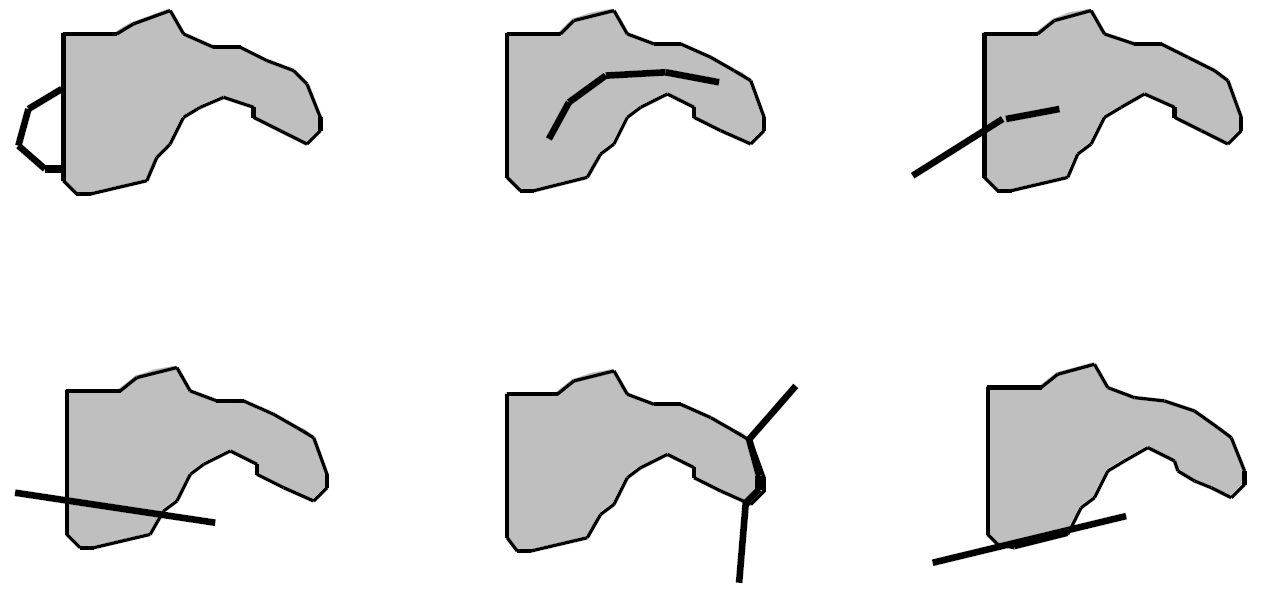
\includegraphics[width=\textwidth]{images/evaluation_setup.png}
		\begin{center}
			Here are six of the diagrams that were used in this research, which are obviously all geometrically distinct. Find the pair that is topologically identical.
			\textcolor{white}{\textbf{Answer:} The right and middle examples in the lower row are topologically identical but geometrically distinct.}
		\end{center}
	}
	
	\only<2>
	{
		\centering 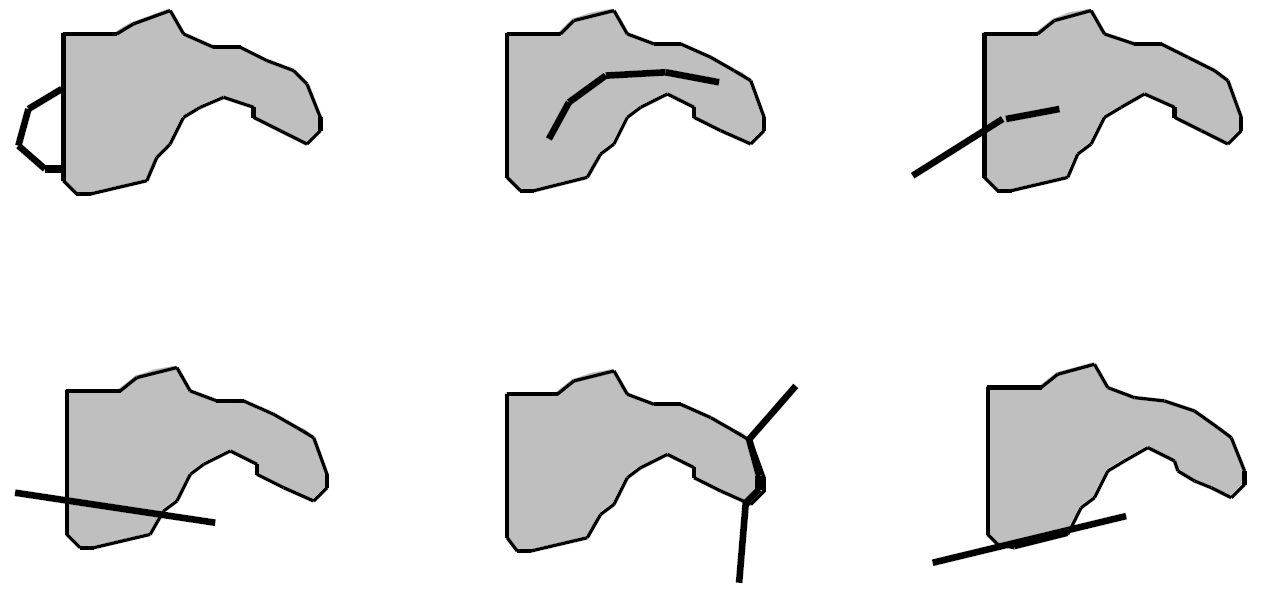
\includegraphics[width=\textwidth]{images/evaluation_setup.png}
		\begin{center}
			\textbf{Answer:} The right and middle examples in the lower row are topologically identical but geometrically distinct.
		\end{center}
	}
\end{frame}

\begin{frame}{Task}
	\begin{itemize}
		\item group spatial relations between line and region, road and park (parks were all the same size and shape)
		\item arrange the sketches into several groups, such that you would use the same verbal description for the spatial relationship between the road and the park for every sketch in each group
		
	\end{itemize}
\end{frame}

\begin{frame}{Goal}
	\begin{block}{Goal}
		\begin{itemize}
			\item analyse how the subjects formed groups of similar relations
			\item check similarity with presented conceptual neighborhood models
		\end{itemize}
	\end{block}
\end{frame}


\begin{frame}{Results}
	\begin{itemize}
		\item The pairs that were neighbors by both snapshot and smooth-transition models were grouped from 0 to 78 times, with a mean of 33.6.
		
		\item Those pairs that were neighbors for smooth transitions-but not snapshots- were grouped between 0 and 66 times, with a mean of 17.3 (15.4 per cent).
		
		\item The two pairs that were snapshot neighbors-but not smooth transition neighbors- were grouped 10 and 16 times (mean = 14; 11.6 per cent).
		
		\item Perhaps most significant, however, is the fact that the 131 pairs that were neighbors by neither the snapshot model nor the smooth transitions were grouped an average of only 6.0 times by the subject (5.3 per cent of the maximum).
		
		\item Sixty pairs were never grouped by any of the 28 subjects nor any of the four possible stimulus pairs. The most frequently-grouped pair in this category was 54 times (48 per cent), but only 20 stimulus pairs with neither smooth transitions nor minimum snapshot difference were grouped 12 or more times (10 per cent of the maximum).
		
		\item 
	\end{itemize}
	%	\begin{itemize}
	%		\item \textbf{task:} 
	%		
	%		
	%		\item Goal: Within the context of different models for conceptual neighbors, it is particularly enlightening to analyse how the subjects formed groups of similar relations.'
	%		
	%		\item 28 subjects performing tasks
	%		
	%		\item each spatial relation could be grouped as many as 112 times (4 pairs times 28 subjects) with each other relation
	%	\end{itemize}
\end{frame}
